
\section{Presentación de la asignatura}

%%---------------------------------------------------------------

\begin{frame}
\frametitle{Datos, datos, datos}

\begin{itemize}
\item Profesores:
  \begin{enumerate}
  \item Jesús M. González Barahona (jgb @ gsyc.urjc.es)
  \item Gregorio Robles (grex @ gsyc.urjc.es)
  \end{enumerate}
\item Grupo de Sistemas y Comunicaciones (GSyC)
\item Despachos: 101 y 110 Departamental III
\item Tutoría: X de 16:00 a 19:00 (en los propios Laboratorios)
\item Horario: \horario
\item Laboratorio 209 Laboratorios III (habitualmente)
\end{itemize}

\begin{flushright}
Campus virtual: {\small \url{http://aulavirtual.urjc.es/}} \\
Materiales: {\small \url{http://cursosweb.github.io/}} \\
%% Acortador: {\small \url{http://pili.la/dat15}}
\end{flushright}

\end{frame}


%-----------------------    ---------------------------------
\usebackgroundtemplate{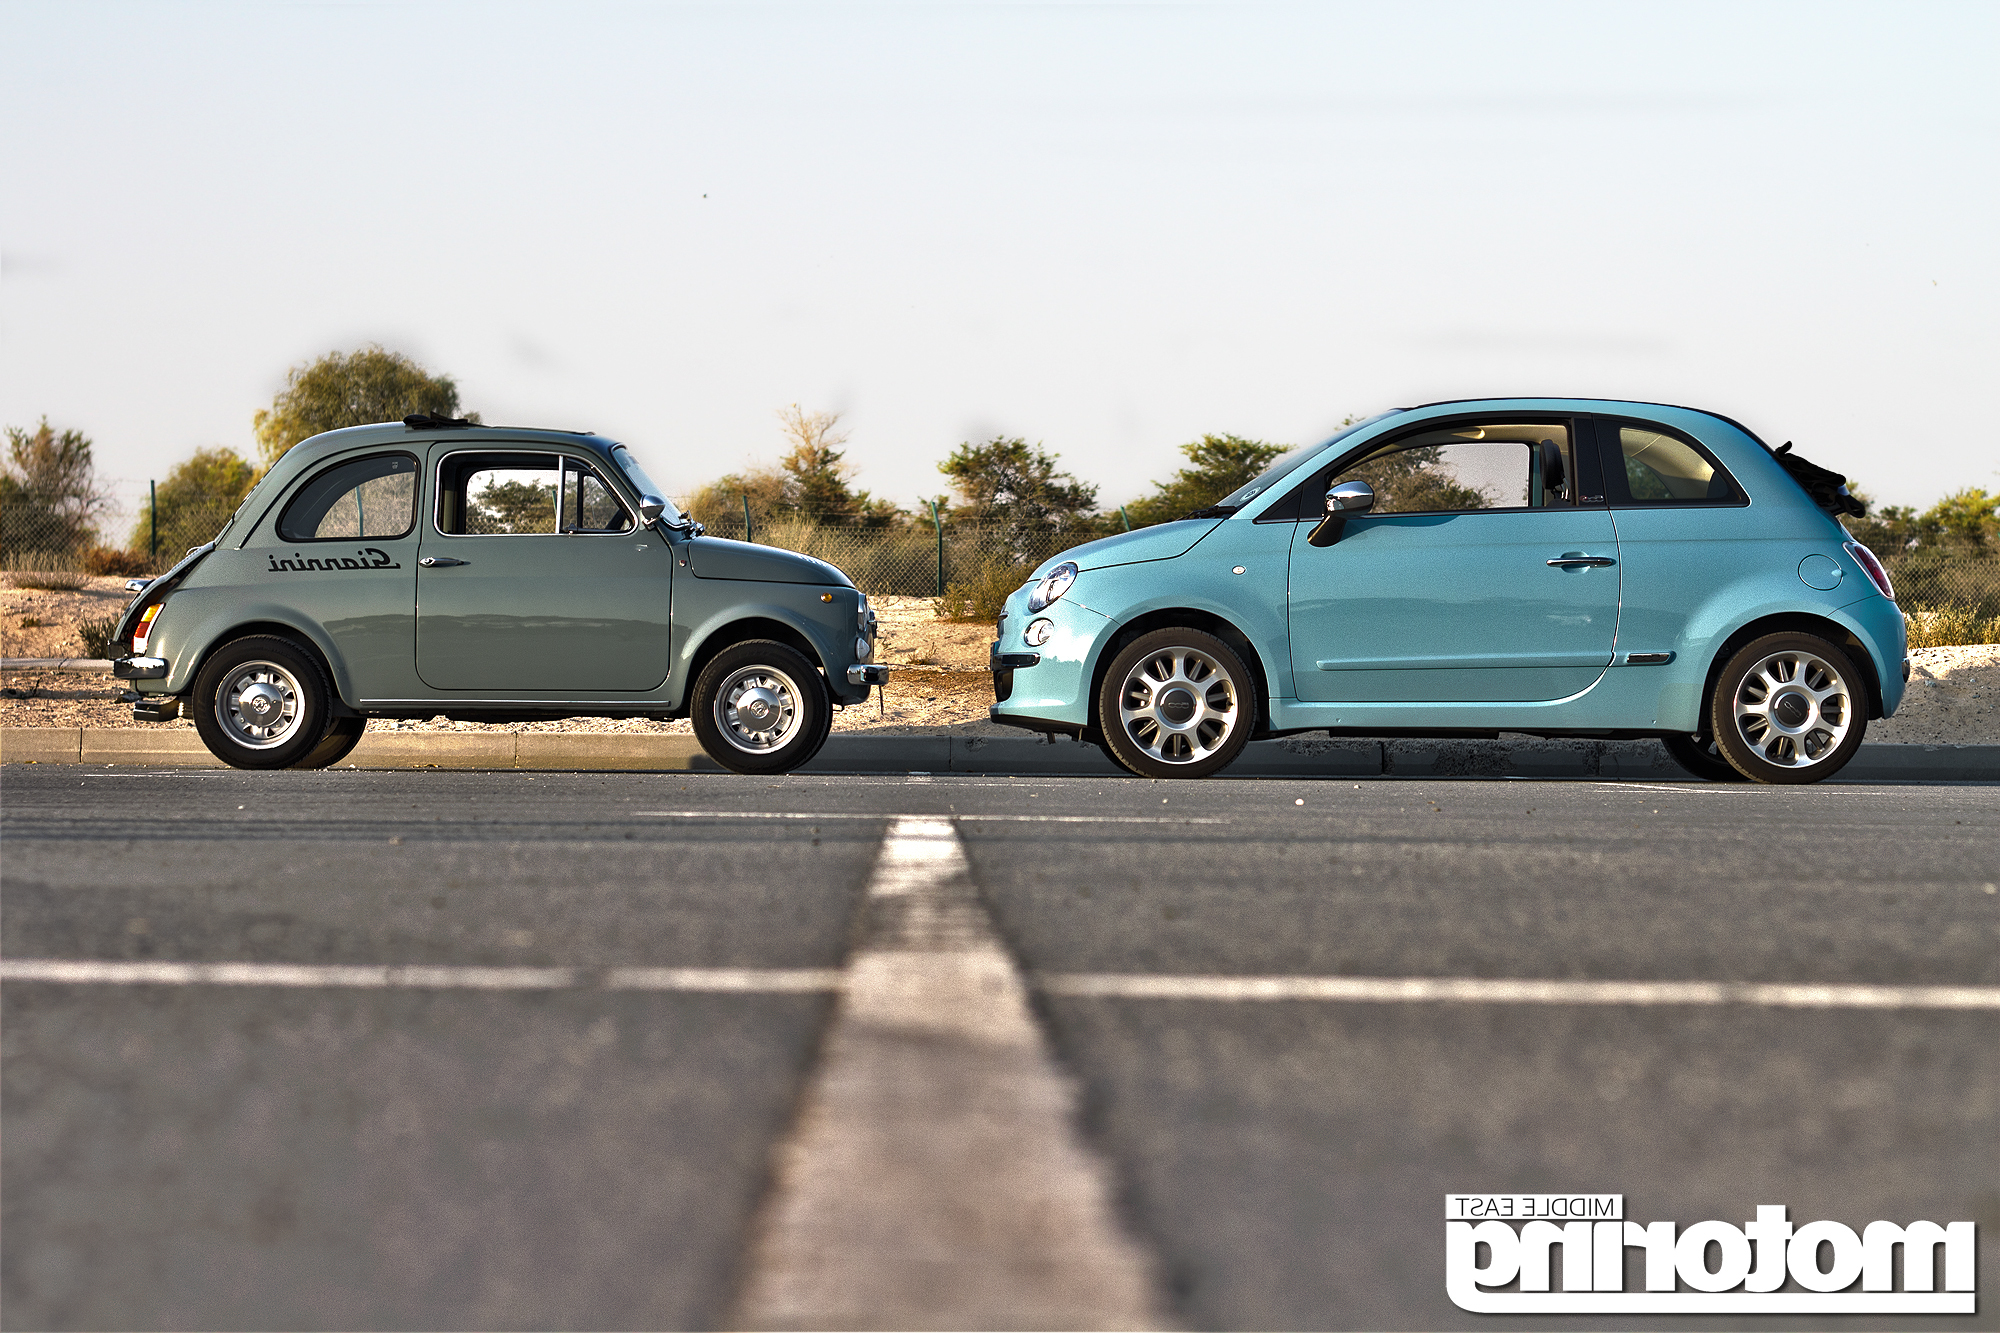
\includegraphics[width=12.8cm]{figs/oldnew.jpg}}
% 

\begin{frame}
\frametitle{¿De qué va todo esto?}

\vspace{3cm}

\begin{center}
\Huge El \emph{viejo} Internet ya no nos vale
\end{center}

\end{frame}
\usebackgroundtemplate{}


%%---------------------------------------------------------------

\begin{frame}
\frametitle{En concreto...}


\begin{itemize}
\item HTML, HTML5
\item CSS, CSS3, Bootstrap
\item JavaScript
\item Canvas, WebWorkers, WebSockets...
\item Video, Audio
\item Geolocalización
\item WebGL, WebVR
\item APIs
\item \dots
%% \item Cómo se construyen los sistemas reales que se usan en Inet
%% \item Qué tecnologías se están usando
%% \item Qué esquemas de seguridad hay
%% \item Cómo encajan las piezas
%% \item En la medida de lo posible, ``manos en la masa''.
\end{itemize}


\end{frame}

%-----------------------    ---------------------------------
\usebackgroundtemplate{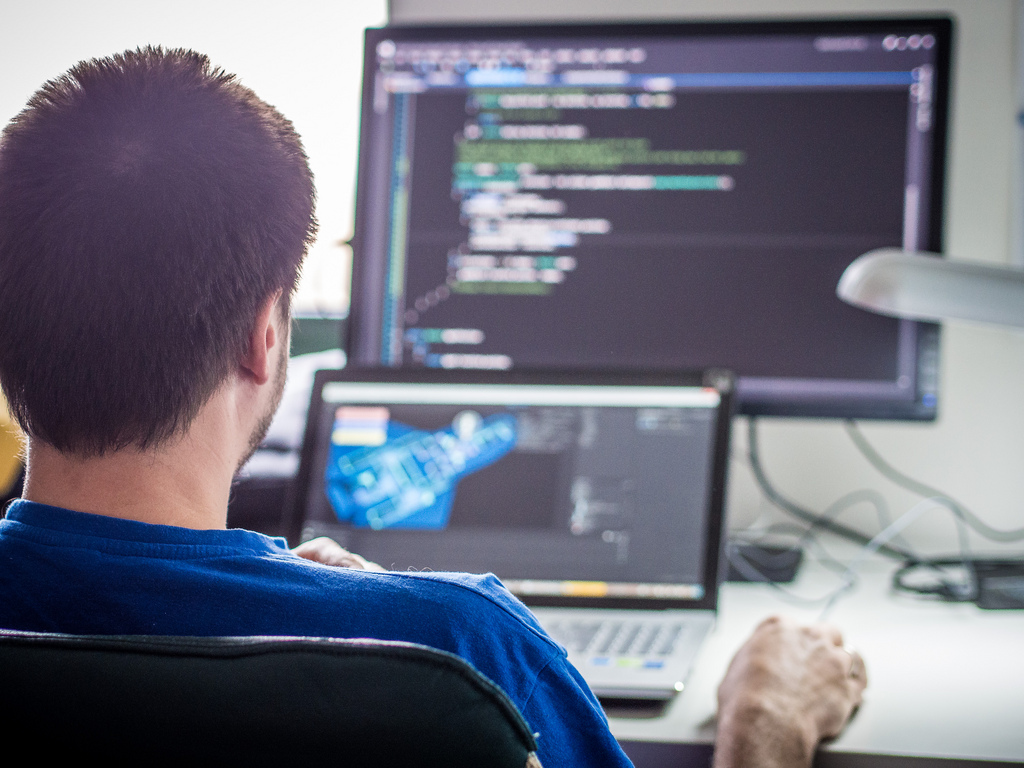
\includegraphics[width=13cm]{figs/programmer.jpg}}
% http://www.openweigh.com/assets/programmer-e898f9c9a43ecd208f1f1df347713e6e.jpg

\begin{frame}
\frametitle{Fundamentos ``filosóficos''}

\vspace{2.7cm}

\begin{center}
{\Huge \bf La programación es el lenguaje de la tecnología}
\end{center}

\end{frame}
\usebackgroundtemplate{}

%-----------------------    ---------------------------------

\begin{frame}
\frametitle{Lenguaje de Programación: JavaScript}

\begin{center}
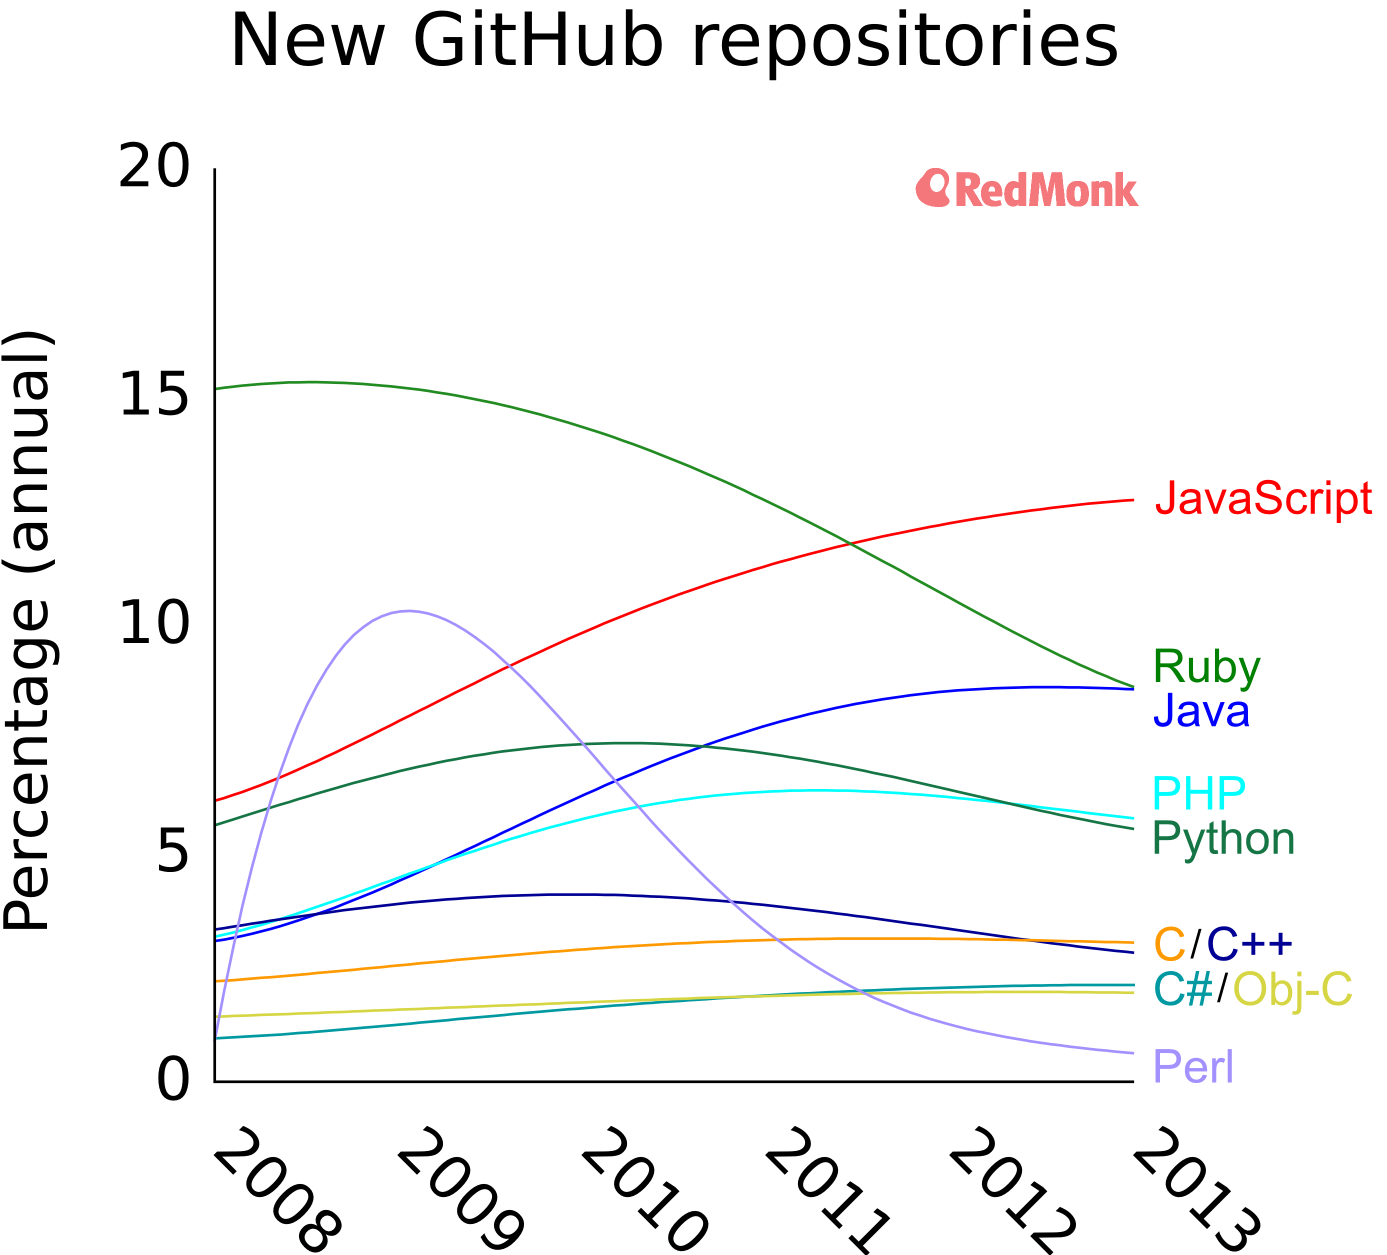
\includegraphics[width=6cm]{figs/2013-most-popular-on-github.png}
\end{center}

\begin{center}
\Large Primer Mandamiento: \\ Amarás JavaScript por encima de (casi) todo.
\end{center}


\end{frame}
\usebackgroundtemplate{}


%%---------------------------------------------------------------

\begin{frame}
\frametitle{Ejemplos}

\begin{itemize}
  \item Utilizando Google Maps para ver las antípodas \\ \url{http://www.antipodesmap.com/}
  \item Pintando en el Canvas \\ \url{http://www.williammalone.com/articles/create-html5-canvas-javascript-drawing-app/}
  \item Transiciones CSS3 \\ \url{http://css3.bradshawenterprises.com/transitions/}
  \item Creando un Comecocos \\ \url{https://github.com/platzhersh/pacman-canvas}
  \item Creando webs modernas y adaptable \\ \url{http://gsyc.es/~grex/leonardo/}
  \item ...
\end{itemize}

\end{frame}



%%---------------------------------------------------------------

\begin{frame}
\frametitle{Metodología}

{\Large
\begin{itemize}
\item Objetivo principal: conceptos básicos de construcción de aplicaciones HTML5 portables
\item Clases de teoría y de prácticas, pero...
\item ...teoría en prácticas, prácticas en teoría
\item Uso de resolución de problemas para aprender
\item Fundamentalmente, entender lo fundamental
\end{itemize}
}

\end{frame}

%-----------------------    ---------------------------------
\usebackgroundtemplate{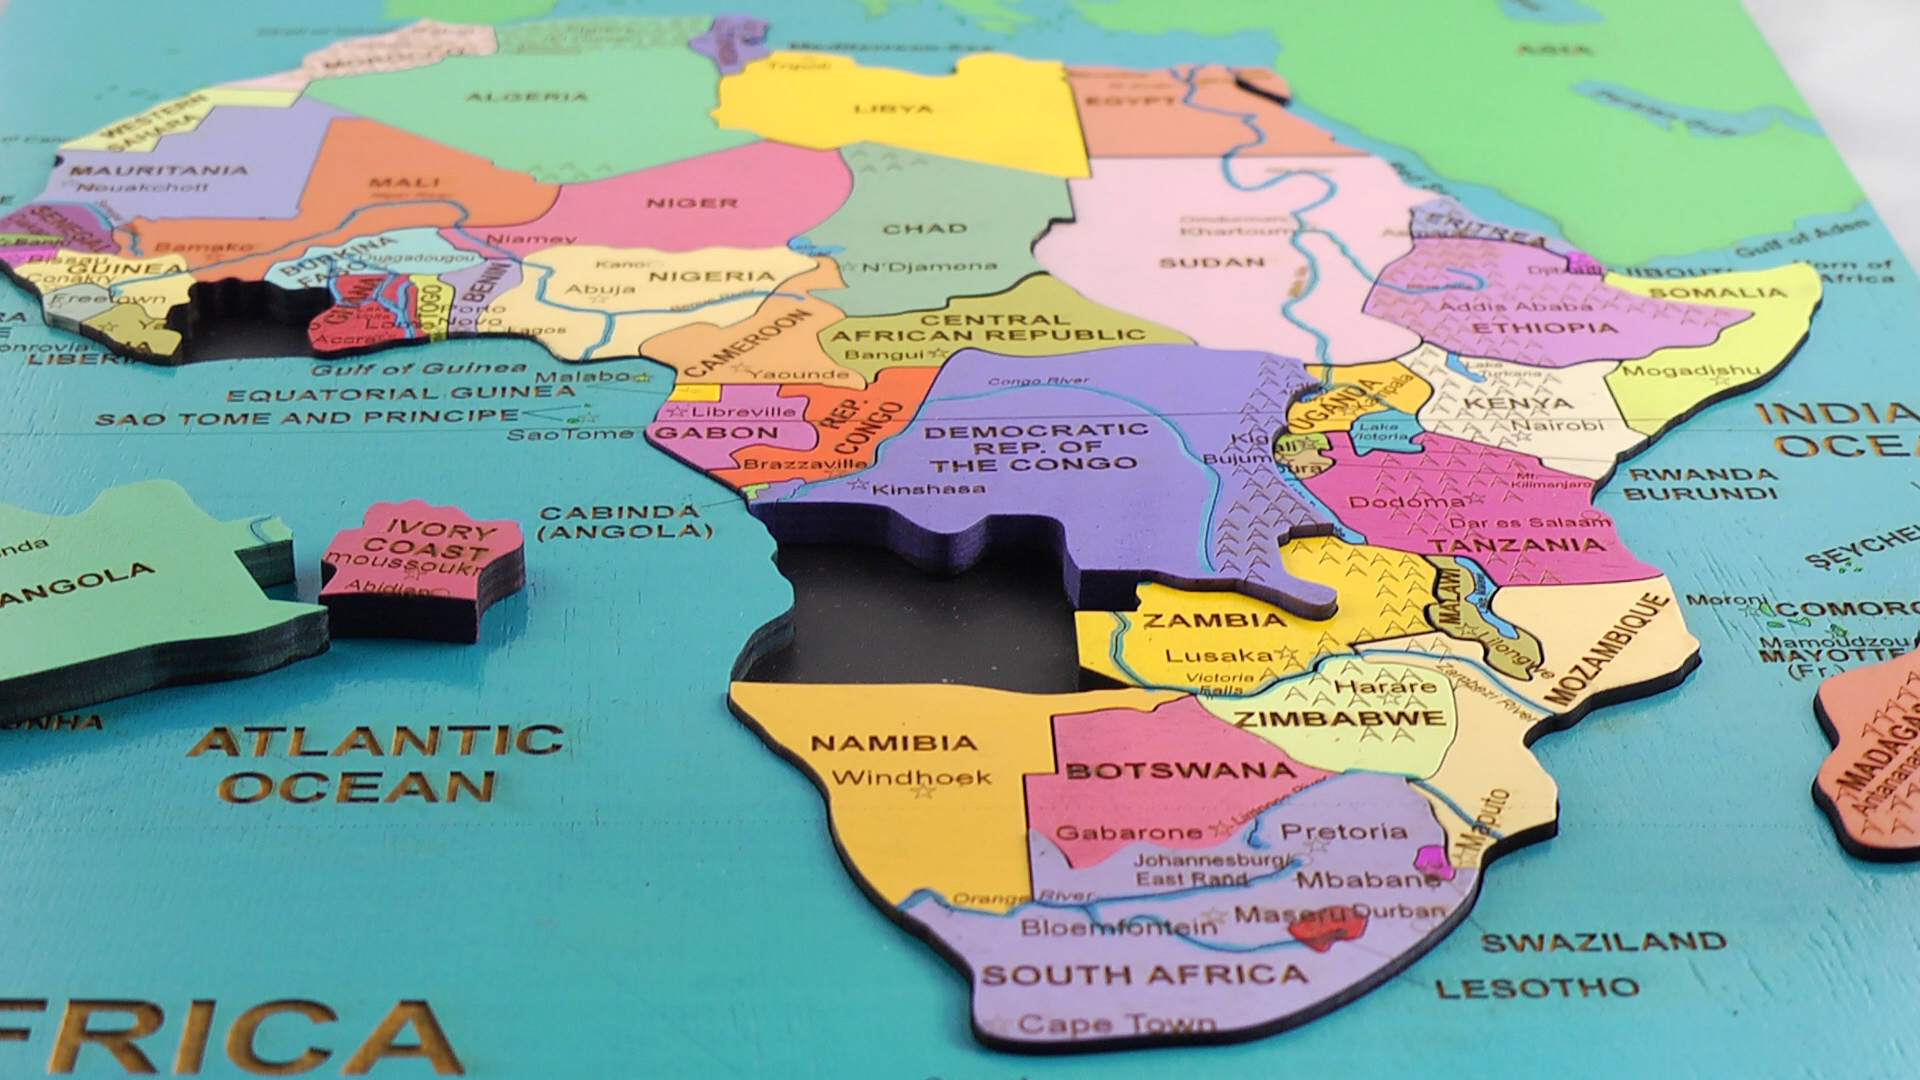
\includegraphics[width=13cm]{figs/africa.jpg}}
% http://www.funlearningcompany.com/wp-content/themes/smallbiz/images/Map100.jpg

\begin{frame}
\frametitle{Fundamentos ``filosóficos''}

\vspace{5.4cm}

\begin{center}
\Huge Aprender no puede ser aburrido
\end{center}

\end{frame}
\usebackgroundtemplate{}

%%---------------------------------------------------------------

\begin{frame}
\frametitle{Las Clases}

{\Large
\begin{itemize}
  \item Empezamos a las 13:00 en punto
  \item 10 minutos con un tema motivacional
  \begin{itemize}
    \item Gadgets tecnológicos
    \item Aplicaciones
    \item Cuestiones interesantes
    \item \dots
  \end{itemize}
  \item Generalmente, explicación de los conceptos más importantes y luego
realización de ejercicios
  \item No hay descanso
  \item Ejercicios para hacer fuera de clase (y entregar)
\end{itemize}
}
\end{frame}



%-----------------------    ---------------------------------
\usebackgroundtemplate{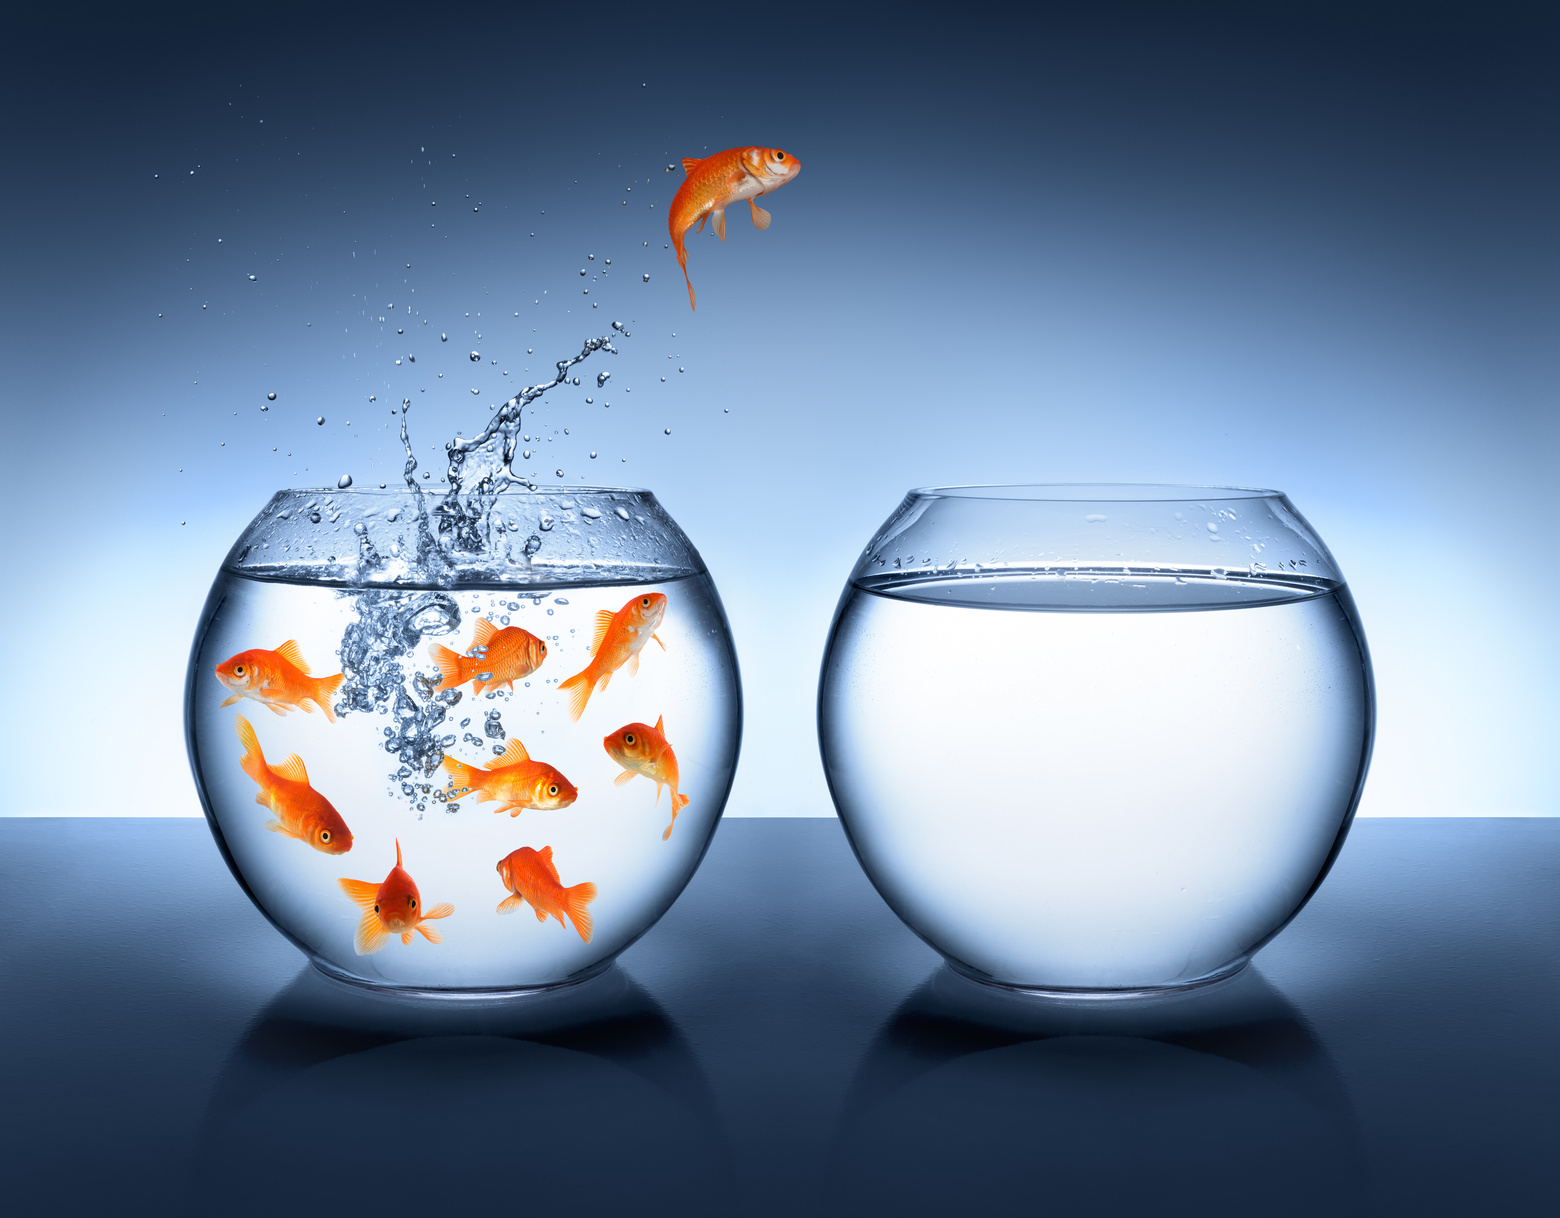
\includegraphics[width=13.5cm]{figs/challenge.jpg}}
% http://ichallenge.com/wp-content/uploads/2014/08/challenge-6.jpg

\begin{frame}
\frametitle{Fundamentos ``filosóficos''}

\vspace{-2.75cm}

\begin{center}
\Huge El estudiante es el centro del aprendizaje
\end{center}

\end{frame}
\usebackgroundtemplate{}



%%---------------------------------------------------------------

\begin{frame}
\frametitle{Evaluación}

\begin{itemize}
\item Microprácticas diarias (entrega foro/GitHub): 0 a 1
\item Miniprácticas preparatorias: 0 a 2
\item Práctica final (obligatorio): 0 a 2.
\item Opciones y mejoras práctica final: 0 a 3
\item Teoría (obligatorio): 0 a 4.
\item Nota final: Suma de notas, moderada por la interpretación del profesor
\item Mínimo para aprobar:
      \begin{itemize}
      \item Aprobado en teoría (2) y práctica final (1), y
      \item 5 puntos de nota final en total
      \end{itemize}
\end{itemize}

\end{frame}

%%---------------------------------------------------------------

\begin{frame}
\frametitle{Evaluación (2)}

\begin{itemize}
\item Evaluación teoría: prueba escrita
\item Microprácticas diarias y miniprácticas incrementales:
      \begin{itemize}
      \item es muy recomendable hacerlas
      \end{itemize}
\item Evaluación práctica final
      \begin{itemize}
      \item posibilidad de examen presencial para práctica final
      \item ¡tiene que funcionar en el laboratorio!
      \item enunciado mínimo obligatorio supone 1, se llega a 2 sólo con calidad y cuidado en los detalles
      \end{itemize}
\item Opciones y mejoras práctica final:
      \begin{itemize}
      \item permiten subir la nota mucho
      \end{itemize}
\item Evaluación extraordinaria:
  \begin{itemize}
  \item prueba escrita (si no se aprobó la ordinaria)
  \item nueva práctica final (si no se aprobó la ordinaria)
  \end{itemize}
\end{itemize}

\end{frame}

%%---------------------------------------------------------------

\begin{frame}
\frametitle{Ejemplos de prácticas finales de otros años}

\begin{itemize}
  \item Alejandro García - Gascó Pérez: \url{https://www.youtube.com/watch?v=iDS1l1ZE5ak}
  \item Alejandro Campos: \url{https://www.youtube.com/watch?v=rzoK09BjSvI}
  \item Jesús Alonso: \url{https://www.youtube.com/watch?v=3QNGv0rA2cM}
  \item Sandra Álvarez: \url{https://www.youtube.com/watch?v=-6j7FbR-mLc}
\end{itemize}

(puedes buscar en YouTube por muchos más ejemplos)

\end{frame}



%%---------------------------------------------------------------

\begin{frame}
\frametitle{¡Ánimo!}

\begin{center}
{\huge Aquí se enseñan cómo son las cosas \\
  que se usan en el mundo real \\
  ~ \\
  Las buenas noticias son\dots \\
  que no son tan difíciles\\}
\end{center}

\end{frame}


